\documentclass[nobib]{MSword}
% Class options:
%-------------------------------
% nobib         - skip bibliography code/ don't include bib
% math          - include math packages and useful math commands
% hidelinks     - hide hyperref colored link boxes
% wordlinks     - link color scheme similar to word


% Preamble code:
%%%%%%%%%%%%%%%%%%%%%%%%%%%%%%%%%%%%%%%%
\usepackage[english]{babel}
\usepackage{csquotes}
\usepackage{lipsum}

% % Uncomment using "Ctrl + /" (/ on numpad):
% % Customizing headers and footers:
% \fancypagestyle{custom}{%
%     \fancyhf{}% clears the footer and header
%     % Header:
%     \fancyhead[L]{}
%     \fancyhead[C]{}
%     \fancyhead[R]{}
%     % Footer:
%     \fancyfoot[L]{}
%     \fancyfoot[C]{}
%     \fancyfoot[R]{}
%         % Tips:
%         % ----
%         % L: left, C: center, R: right
%         % O: odd pages, E: even pages
%         % ----
%         % Example: \fancyghead[LO,RE]{Text}
%         % will produce "Text" left in the header
%         % on odd pages and right in the header on even pages.
%     % Rules/ lines:
%     \renewcommand{\headrulewidth}{0.4pt}
%     \renewcommand{\footrulewidth}{2pt}
% }
% % Changing the pagestyle:
% \pagestyle{custom}

%%%%%%%%%%%%%%%%%%%%%%%%%%%%%%%%%%%%%%%%

% Preamble information:
%%%%%%%%%%%%%%%%%%%%%%%%%%%%%%%%%%%%%%%%

\title{Fourier Series Approximation of a Sqaure Wave}
\author{Dre Mata}
\date{20 March 2023}

%%%%%%%%%%%%%%%%%%%%%%%%%%%%%%%%%%%%%%%%

% The document:
%%%%%%%%%%%%%%%%%%%%%%%%%%%%%%%%%%%%%%%%
\begin{document}

\maketitle
\begin{center}
    Part 1:
\end{center}
The objective of this lab is to approximate periodic time-domain signals using Fourier Series. This is done by first finding the ak and bk constants in the prelab. It was found that the ak constant came out to be equal to zero. The bk constant comes out to be equal to the constant shown below.

\begin{center}
    $bk = [2/(k*pi)]*[1 - cos(k*pi)]$
\end{center}

\begin{center}
    $ak = 0$
\end{center}

After this was completed python was used to find the a0, a1, b1, b2, and b3 values. The values can be seen in Figure one. After this was done the values were plugged into the Fourier series formula and were plotted. The sample sizes for these plots were 1, 3, 15, 50, 150, 1500. The plots can be seen in Figures two, three, four, five, six, and seven respectively. 



\begin{center}
    Questions:
\end{center}

1. Is x(t) an even or an odd function? Explain why.

X(t) is odd, because it straddles -T and T in such a way that the integral of X(t) from -T to T would result in zero. This means the function is odd.

2. Based on your results from Task 1, what do you expect the values of a2, a3, ...., an to be why?

I expect the values of a2, a3, ...., an to be zero. This is because the function for ak was 0, this means there could be no other possible value.

3. How does the approximation of the square wave change as the value of N increases? In what way does the Fourier series struggle to approximate the square wave?

As N increases the function becomes more like a Square wave. There are two ways this Fourier series struggles to approximate the square wave. The first is that if N is too small the resolution of the function will be poor. If the N is big the resolution will be better, but it will take more computing power. The Second struggle is Gibbs phenomenon. This being that there are discontinuities in our function there will be a spike in the function right before and after. This will smooth out however as N increases, but will always be there.

4. What is occurring mathematically in the Fourier series summation as the values of N increases?

As N increases there are more terms in the Fourier series summation.



\begin{center}
    Figures
\end{center}

Figure 1:

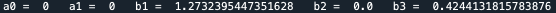
\includegraphics[scale = 0.75]
{txt/Lab8Fig1.png}

Figure 2:

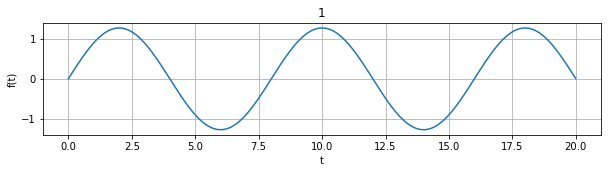
\includegraphics[scale = 0.75]
{txt/Lab8Fig2.png}

Figure 3:

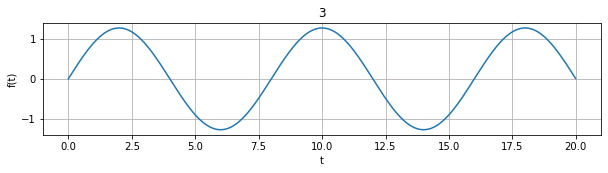
\includegraphics[scale = 0.75]
{txt/Lab8Fig3.png}

Figure 4:

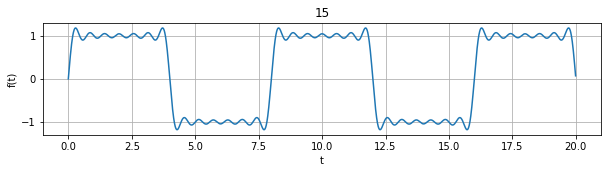
\includegraphics[scale = 0.75]
{txt/Lab8Fig4.png}

Figure 5:

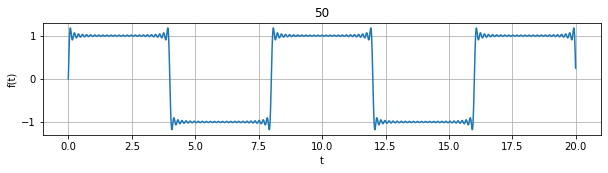
\includegraphics[scale = 0.75]
{txt/Lab8Fig5.png}

Figure 6:

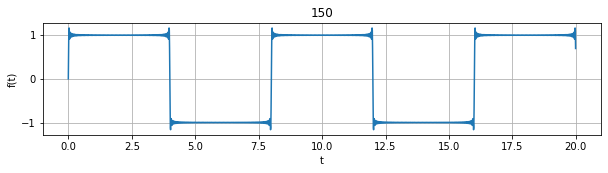
\includegraphics[scale = 0.75]
{txt/Lab8Fig6.png}

Figure 7:

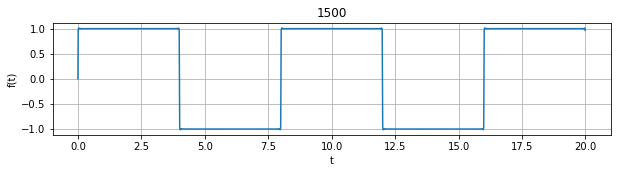
\includegraphics[scale = 0.75]
{txt/Lab8Fig7.png}


\begin{center}
    Conclusion
\end{center}
    This lab helped me gain a better understanding on how Fourier series are used to approximate periodic time-domain signals. Python helped me gain a better understanding on what functions look like with more terms and fewer terms in the Fourier series.

\end{document}
%%%%%%%%%%%%%%%%%%%%%%%%%%%%%%%%%%%%%%%%

% Copyright Remarks:
%--------------------

% Copyright holder: Vebjørn S. Førde, copyright: CC BY 4.0
% Note: The author of this template is also the copyright holder.

% Below is an explanation of the CC BY 4.0. Additional statements/ 
% clarifications made by the author/copyright holder are marked with *.

% YOU ARE FREE TO:
% Share — copy and redistribute the material in any medium or format
% Adapt — remix, transform, and build upon the material
% for any purpose, even commercially.

% UNDER THE FOLLOWING TERMS:
% Attribution* — You must give appropriate credit, provide a link to the license,
% and indicate if changes were made. You may do so in any reasonable manner, but 
% not in any way that suggests the licensor endorses you or your use.

% *Note: 
% Attribution NOT NEEDED for: 
%       - PDF distibution (like sharing your PDF document)
%       - Use of (dummy)text and images provided in the template (obviously)
%       - Distributing parts of the template, and not the template as a whole
% I am not really concerned with being given credit. As long as you do not 
% claim to have made the template yourself in distributing it further, I have
% no complaints.

% No additional restrictions — You may not apply legal terms or technological 
% measures that legally restrict others from doing anything the license permits.

% NOTICES:
% No warranties are given.

% Disclaimer* (added by copyright holder):
% THE SOFTWARE IS PROVIDED "AS IS", WITHOUT WARRANTY OF ANY KIND, EXPRESS OR
% IMPLIED, INCLUDING BUT NOT LIMITED TO THE WARRANTIES OF MERCHANTABILITY,
% FITNESS FOR A PARTICULAR PURPOSE AND NONINFRINGEMENT. IN NO EVENT SHALL THE
% AUTHORS OR COPYRIGHT HOLDERS BE LIABLE FOR ANY CLAIM, DAMAGES OR OTHER
% LIABILITY, WHETHER IN AN ACTION OF CONTRACT, TORT OR OTHERWISE, ARISING FROM,
% OUT OF OR IN CONNECTION WITH THE SOFTWARE OR THE USE OR OTHER DEALINGS IN THE
% SOFTWARE.

% Read more about CC BY 4.0:
% https://creativecommons.org/licenses/by/4.0/